\documentclass{article}
\usepackage[utf8]{inputenc}
\usepackage{polski}
\usepackage{multirow}
\usepackage[margin=2.5cm]{geometry}
\usepackage{amsmath}
\usepackage{graphicx}

\title{Programowanie Obiektowe i Graficzne\\
Projekt zespołowy\\
\textbf{FilterStudio}}
\author{Skład zespołu projektowego: \\ Paweł Chłąd\\Daniel Jambor\\ Bartek Meller }

\begin{document}

\maketitle

\begin{center}
    \begin{tabular}{ |c|c|c| }
        \hline
        Imię Nazwisko                   & Odpowiedzialny za                        & Zrealizował zadania                      \\ \hline
        \multirow{3}{*}{Paweł Chłąd}    &                                          & 1A. Rozplanowanie architektury           \\
                                        & Architekurę aplikacji                    & 1B. Implementacja architektury aplikacji \\
                                        &                                          & 1C. Implementacja filtrów konwolucyjnych \\ \hline
        \multirow{2}{*}{Daniel Jambor}  & UI/UX                                    & 2A. Projektowanie UI/UX                  \\
                                        &                                          & 2B. Wdrożenie założeń UI/UX              \\ \hline
        Bartek Meller                   & Walidacja danych i dodatkowe elementy UI & 3A. Walidacja wprowadzanych danych      \\ 
                                        &                                          & 3B. Dodatkowe kontrolki użytkownika    \\ \hline
    \end{tabular}
\end{center}

\pagebreak


\section{Opis projektu}
FilterStudio to aplikacja pozwalająca na budowanie systemów filtrów do zdjęć. Najczęściej są to filtry konwolucyjne, ale architektura aplikacji pozwala
na dołączanie innych rodzajów filtrów. Użytkownik może wprowadzić zdjęcie i zmodyfikować je za pomocą filtrów.
\section{Wymagania}
Projekt spełnia następujące założenia funkcjonalne:
\begin{itemize}
    \item Użytkownik może budować filtry konwolucyjne
    \item Użytkownik może składać wiele filtrów w jeden \textit{projekt}
    \item Użytkownik może zapisać projekt, wraz z konfiguracjami filtrów
    \item Użytkownik może wprowadzić obraz do programu aby poddać go obróbce filtrom
    \item Użytkownik może zapisać przefiltrowany obraz 
\end{itemize}

Założenia niefunkcjonalne są następujące:
\begin{itemize}
    \item Solidna architektura aplikacji pozwalająca na łatwe wprowadzanie nowych filtrów do programu
    \item Szybkie wykonywanie filtrów konwolucyjnych poprzez użycie surowego dostępu do danych bitmapy
\end{itemize}


\section{Przebieg realizacji}
%Każdy z wykonawców opisuje wykonane przez siebie zadania. Należy zamieścić ewentualnie schemat bazy danych (gdy aplikacja jest bazodanowa), opis algorytmu, gdy aplikacja jest związana z SSI lub inną algorytmiką. W przypadku zastosowania wzorców projektowych proszę to tu podkreślić. Należy też zwrócić uwagę na architekturę aplikacji tzn. jeśli używacie MVVM to podkreślamy tu to.
%W miejscu tym należy opisać interfejs publiczny stworzonych w ramach projektu klas. Mile widziane diagramy uml.

\subsection{Architektura}
Aplikacja została z góry zaprojektowana tak, aby współgrała ze wzorcem MVVM. Ważnym było też zapewnienie rozszerzalności projektu o dodatkowe rodzaje filtrów i 
możliwości budowania owych filtrów. Aby wspierać różne rodzaje filtrów, posłużyliśmy się wzorcem \textbf{strategii}, zamknęliśmy filtry za jednolitym interfejsem, dzięki czemu
mogliśmy napisać obsługę wielu rodzajów filtrów. Później w trakcie prac okazało się iż potrzebujemy sposobu na dostarczanie \textit{różnych} danych do \textit{różnych} typów filtrów.
Problem rozwiązaliśmy poprzez wprowadzenie \textbf{fabryki abstrakcyjnej}, dzięki czemu mogliśmy, tak samo jak w przypadku strategii, posługiwać się interfejsem
do różnych fabryk, zamiast używać konkretnych obiektów. Następnym problemem było dostarczanie użytkownikom sposobu zmiany istniejących już filtrów (fabryka rozwiązuje tylko problem kreowania ich),
zostało rozwiązane to poprzez użycie klasy abstrakcyjnej \textbf{FilterDataProviderVM}, która służy jako baza dla klas ViewModel, mających obsługiwać interakcję użytkownika z 
danymi filtrów. Każdy FilterDataProviderVM jest pewnym sposobem dzięki któremu dane mogą trafić do filtra. Do jednego typu filtra może nawet być przypisane wiele
sposobów dostarczania danych, np. filtr gaussowski nadal jest filtrem konwolucyjnym, nie miałoby sensu tworzyć osobnej klasy filtra, który robi to samo co zwykły
filtr, ale filtr gaussowski tworzymy inaczej niż filtr zwykły (poprzez określenie parametrów takich jak odchylenie standardowe). Naturalnym więc było, dostarczenie klas
odpowiedzialnych tylko za tworzenie i przekazywanie danych do filtrów.

\subsection{Filtry Konwolucyjne}
Filtr konwolucyjny jest podstawą programu. Jego budowa i działanie są następujące:

Filtr składa się z macierzy 2D, która reprezentuje \textit{maskę} filtru:

\begin{gather}
    F = 
       \begin{vmatrix}
        f_{11} & f_{12} & f_{13}\\
        f_{21} & f_{22} & f_{23}\\
        f_{31} & f_{32} & f_{33}\\
        \end{vmatrix}
\end{gather}

Obraz to tak naprawdę macierz pixeli, którą oznaczymy jako $I$.
Proces nakładania filtru wygląda następująco:

\begin{gather}
    F * I = \sum_{dx = -a}^{a} \sum_{dy = -b}^{b} f_{dxdy} \cdot i_{x+dx, y+dy}
\end{gather}

Gdzie x i y to pixel obrazu który będzie zmieniony po tej operacji. Cała operacja $F*I$ 
zwróci nam obraz po przejściu przez filtr. Jak wiemy obrazy nie składają się tylko 
z jednego koloru (u nas RGB) więc tą operację powtarzamy dla wszystkich kanałów osobno.

W naszej implementacji zastosowaliśmy także normalizację która opiera się na prostym dzieleniu
przez sumę wszystkich elementów filtra. Dzięki temu z filtrem, który nie jest zbalansowany (czyli jego suma
nie jest równa 0) nie otrzymujemy prześwietlonych/przyciemnionych obrazów.

Przy używaniu filtrów konwolucyjnych pojawia się problem brzegów. W naszej implementacji pomijamy
piksele które wychodzą poza obszar obrazu.


\subsection{User interface}
Utworzenie sprawnego UI okazało się niemałym problemem już w pierwszych wersjach aplikacji. Aplikacja, która jest skomplikowana w samych założeniach wymagała interfejsu, który nie tylko nie odstraszy użytkownika od aplikacji, ale też zachęci go do uczenia się jej. Aplikacja tego typu musiała mieć interfejs który spełniał 3 podstawowe warunki:
\begin{itemize}
	\item Przejrzystość
	\item Prostota
	\item Estetyczność
\end{itemize}
Filter Studio zawiera 3 główne panele, które są jasno opisane i informują użytkownika o ich celu. Zdecydowaliśmy się na podział pionowy, który jest dzisiaj powszechnie stosowany m.in w aplikacjach mobilnych i mocniej wpływa na pozytywny odbiór aplikacji niż podział poziomy. UI zostało również zaprojektowane tak, aby lokalizacja językowa (na ten moment jest to język polski i angielski - zależnie od języka systemu operacyjnego użytkownika) nie sprawiała problemów natury estetycznej. UI zostało napisane z wykorzystaniem języka XAML oraz w nielicznych miejscach języka C\#.


\newpage
\section{Instrukcja użytkownika}
%Opis działania stworzonej aplikacji ze zrzutami ekranów ilustrujące sposób działania aplikacji.

Ta sekcja dostarcza informacji na temat użycia programu \textbf{\textit{FilterStudio}}
\subsection{Overview}

\bigskip
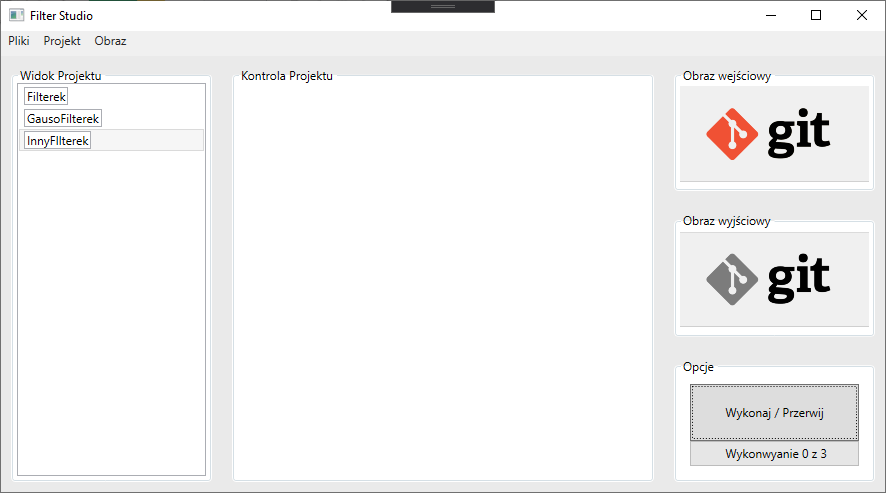
\includegraphics[width=0.9\textwidth]{overview.png}

\begin{itemize}
    \item \textit{Widok Projektu} -- Wyświetla wszystkie aktywne filtry i umożliwia użytkownikowi wybór filtra do edycji
    \item \textit{Kontrola Projektu} -- Umożliwia edycję filtrów, zobacz sekcje "Filtr Gaussa" oraz "Filtr Podstawowy"
    \item \textit{Obraz Wejściowy} -- Wyświetla miniaturę załadowanego obrazu
    \item \textit{Obraz Wyjściowy} -- Wyświetla miniaturę przetworzonego obrazu
    \item \textit{Opcje} -- Ta sekcja zawiera przycisk umożliwiający renderowanie oraz wskaźnik postępu
\end{itemize}

\newpage
\subsection{Filtr Gaussa}
Aby dodać Filtr Gaussa wybierz \textbf{Projekt $\rightarrow$ Dodaj Filtr $\rightarrow$ Filtr Gaussa},

\bigskip
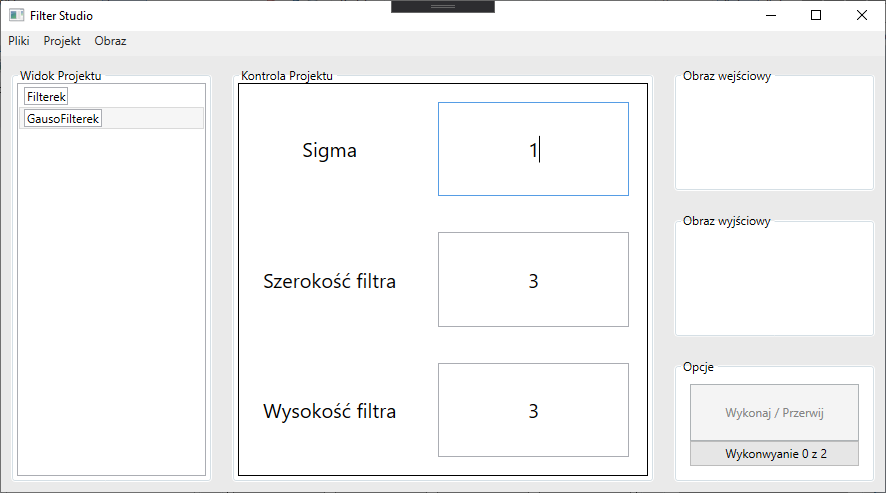
\includegraphics[width=0.9\textwidth]{gauss.png}
\bigskip

i wpisz parametry w pola tekstowe

\subsection{Filtr Podstawowy}
Aby dodać Filtr Podstawowy wybierz \textbf{Projekt $\rightarrow$ Dodaj filtr $\rightarrow$ Podstawowy Filtr},

\bigskip
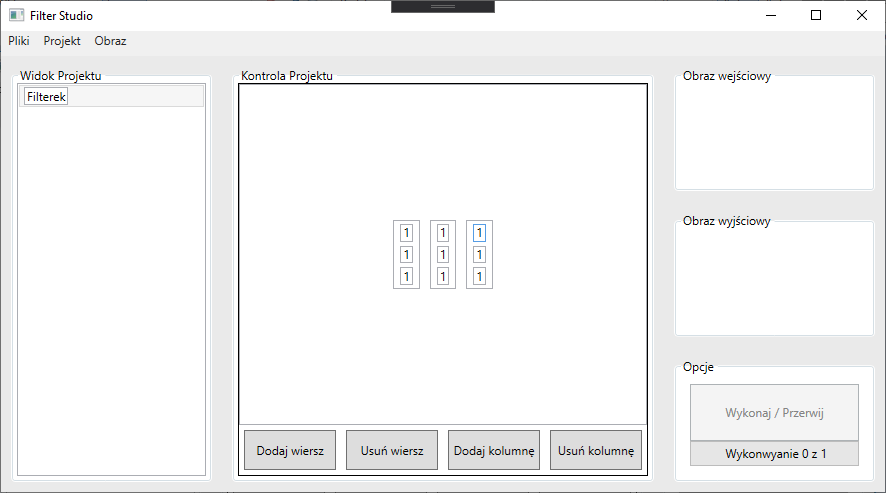
\includegraphics[width=0.9\textwidth]{matrix.png}
\bigskip

dostosuj wymiary macierzy za pomocą przycisków w dolnej części panelu \textbf{Kontroli Projektu} i wpisz wartości w komórki.

\subsection{Filtr czarno-biały}
Aby dodać Filtr czarno-biały wybierz \textbf{Projekt $\rightarrow$ Dodaj filtr $\rightarrow$ Filtr czarno-biały}

\subsection{Wczytywanie, zapisywanie, oraz tworzenie nowych projektów}
Wszystkie te funkcje dostępne są w menu \textbf{Plik} i działają w ustandaryzowany sposób.

\subsection{Wczytywanie i zapisywanie obrazów}
Obie te funkcje dostępne są w menu \textbf{Obraz} i działają w ustandaryzowany sposób.


\section{Podsumowanie i wnioski}
%W miejscu tym piszemy co zrealizowaliśmy, z czym były problemy. Jakie są dalsze kierunki rozwoju tej aplikacji.  
Zrealizowaliśmy pełnoprawny projekt w technologii WPF razem z wdrożeniem wielu wzorców projektowych oraz pomyślnie
wykorzystaliśmy system kontroli wersji \textit{git}.
\subsection{Problemy}
Dużym problemem na początku tworzenia aplikacji było oddzielenie wątku wykonywania filtrów od głównego wątku UI i aplikacji.
Kod wielowątkowy wielokrotnie wyrzucał wyjątki dot. synchronizacji zapisu/odczytu danych ze zmiennych.
Poradziliśmy sobie z problemem poprzez użycie derektyw \textbf{lock} oraz poprzez kopiowanie obiektów bitmap do filtrów 
(tworzyliśmy kopię oryginału znajdującego się w VM), dzięki czemu filtr mógł na osobności operować na bitmapie.

Następnym problemem była optymalizacja filtru konwolucyjnego, problemem były metody GetPixel i SetPixel z klasy Bitmap,
te metody, za każdym razem kiedy zostaną wywołane, wywołują tak naprawdę funkcję w gdiplus.dll poprzez mechanizm P/Invoke.
Przy bitmapie 1000x1000 wywołujemy P/Invoke milion razy!!! (w sumie to dwa bo jeszcze SetPixel)
Problem obeszliśmy poprzez skopiowanie surowych danych bitmapy a następnie operowaliśmy na surowych danych filtrem.
Na koniec kopiujemy wszystkie bajty z powrotem do obiektu bitmapy za pomocą klasy Marshall.
Wszystko by było dobrze, gdyby nie fakt iż długość jednej linii bitmapy jest zawsze wielokrotnością 4 w bajtach.
Więc musieliśmy także uwzględnić padding bitmapy (na szczęście Bitmap udostępnia nam taką informację w właściwości stride)
Nasze rozwiązanie jest około dziesięcio-krotnie razy szybsze od Get/SetPixel.
Najlepszym sposobem przyspieszenia filtrów wszelkiego rodzaju, byłoby jednak użycie
GPU, ale to zostawiamy na przyszłość.



\subsection{Dalszy rozwój}
Opcji na rozwój programu jest dużo:
\begin{itemize}
    \item Przeniesienie operacji filtrów na GPU 
    \item Dodanie nowych filtrów
    \item Dodanie nowych sposobów na tworzenie filtrów
    \item Rozdzielenie kanałów obrazu, możliwość wpływania na dowolny kanał, drzewo filtrów
    \item Możliwość kompilacji drzewa do programu standalone (masowe przetwarzanie zdjęć)
    \item Przetwarzanie filmów (film to seria zdjęć)
    \item Lepsze UI, przeniesienie projektu na bardziej przyszłościową bibliotekę UI
\end{itemize}


\section{Dodatek - udokumentowanie wykorzystania systemu kontroli wersji}
Repozytorium znajduje się pod adresem: https://github.com/Madoxen/FilterStudio
%(może być zrzut/zrzuty ekranu pokazujące, że do realizacji użyliście Państwo systemu kontroli wersji  - wymaga tego efekt E7)

%Uwaga - do dokumentacji proszę nie wklejać całego kodu aplikacji.  W sekcji realizacja można zmieścić fragmenty kodu, jeśli chcecie zwrócić uwagę na coś co było bardzo wymagające i konieczne jest dogłębnego jego omówienia. 
%Poza tym proszę komentować kod aplikacji - to jest istotna część dokumentacji projektu.



\end{document}
